\chapter{User documentation}
In the first part, this chapter introduces a description of the framework itself with all its features. The second part then provides a description of the two showcase games with the way they are controlled.  

\section{Framework}
The TaleCraft framework consists of five main systems whose role is to manage and execute the primary features of a point-and-click adventure game. We will go through each of them and explain the ideal process of creating a game using this framework. The project also includes two scenes that showcase the use of our framework and are located under \verb|Assets > Examples|. In this chapter, we will refer to these two scenes by an abbreviation. The scene from our framework showcasing an area from \textit{Beneath a Steel Sky} (1994) will be referred to as \textit{BaSS}, whereas the one from \textit{The Secret of Monkey Island} (1990) will be called \textit{TSoMI}.

\subsection{Core}
To create a scene using the TaleCraft framework, it must include a \verb|GameObject| with the \textbf{Prefab Manager} component. This component provides a centralized and convenient way to reference prefabs across the framework's scripts. The Prefab Manager relies on a \verb|ScriptableObject| called the \textbf{Prefab Library}, which stores a dictionary of prefabs accessible via string labels. A new Prefab Library asset can be created in the \verb|Assets| folder by right-clicking and selecting \verb|Create > Prefab Library|.

Multiple parts of the framework make use of the Prefab Library to instantiate or reference prefabs. The \verb|Assets/Prefabs| directory contains an instance of the Prefab Library, along with a collection of predefined prefabs tailored for the framework. These prefabs are already referenced within the Prefab Library and are intended to be reused and extended by users of the framework.

\subsection{Walking System}
The walking system is a good starting point right after setting up the the core system. 

\subsubsection{Walkable Map}
The framework provides its own default implementation of the prefab which contains a \verb|GameObject| with \textbf{Walkable Map} script attached to it as a component and by navigating the menu options \verb|GameObject > Walking System| it can be instantiated in the hierarchy. The prefab also comes with a polygon that describes the walkable area accessible to characters. In Figure \ref{fig:Manual-WM}, we can see Unity inspector for the \textbf{Walkable Map} component together with a possible use of this component in scene \textit{BaSS}. An important part of the walking system is the possibility to create obstacles for the player. To do that, the user can simply press at the \textit{Build new polygon obstacle} button, which generates a new \verb|GameObject| with the \textbf{Polygon} component script attached to it (see Figure\ref{fig:Manual-Polygon}). To remove this obstacle from the walking system, one can simply press the button \textit{X} next to the desired polygon in the list of obstacle polygons. 

\begin{figure}[H]
\centering
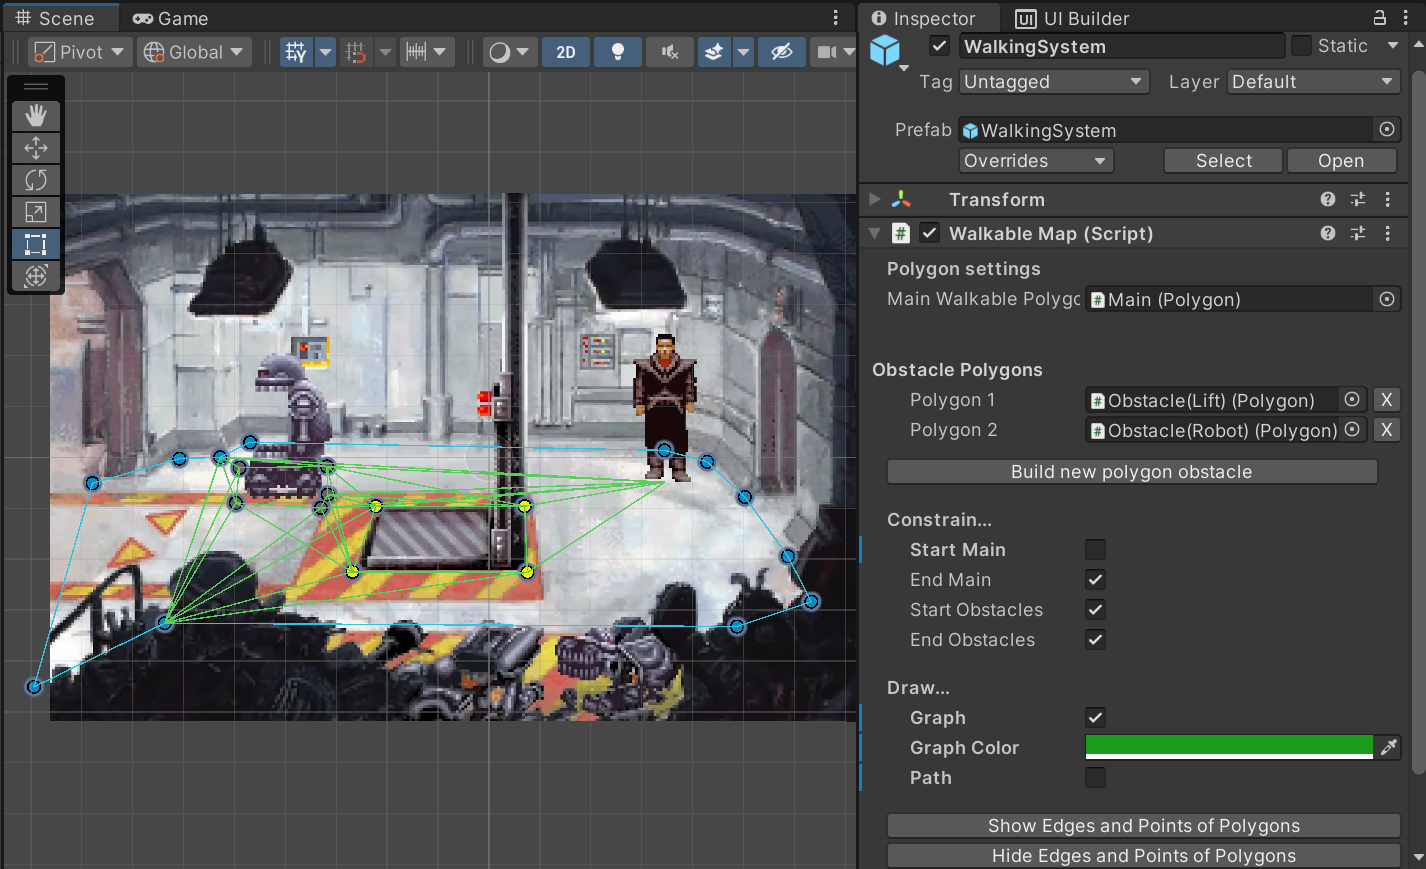
\includegraphics[width=1\linewidth]{img/User doc/walkable_map.png}
\caption{Walkable Map inspector.}
\label{fig:Manual-WM}
\end{figure}

Below that, there are options to constrain the starting or the ending points inside the walkable area and outside the obstacle polygons. In other words, if the player clicks on a point outside the walkable area defined by the developer and the option \textit{End Main} is true, then the system will find the closest possible point in the walkable area from the position of the mouse and will move the character to that point. On the other hand, if false is selected, the character will not move as there is no viable path to the position of the mouse click. Similar rules apply to the \textit{End Obstacles} option, where if a mouse click is registered to be inside an obstacle polygon, the closest possible accessible position is found in the walkable area. The \textit{Start Main} and \textit{Start Obstacle} options work similarly but for the starting position, meaning the character. If the character finds itself to be outside the walkable area and the option \textit{Start Main} or \textit{Start Obstacles} is selected, the character will try to find a way to the given position, otherwise not.

Finally, the component also contains some visual enhancements for the developer. It is possible to visualize the graph created by the polygons and the character with the option to select a desired color for the graph. At the bottom, there is an option to quickly show or hide all edges and points of all polygons contained in this walking system. 

\subsubsection{Polygon}
The Figure \ref{fig:Manual-Polygon} shows an example of an obstacle polygon. The inspector provides some basic visual adjustments to help the developer's workflow. These settings include the visibility of the edges and points together with a color that can be set easily to visually distinguish different polygons from one another. One option also includes the sizing of the points together with a possibility to turn off automatic zooming. \textit{Automatic zooming} (depicted in Figure \ref{fig:Manual-Zoom}) makes the points change size based on the zoom level of the scene. If turned off and zoomed in, the points become very large and the screen is unreadable, so this option is turned on by default.

Undoubtedly, a developer needs to adjust the position and the number of nodes. When the given polygon is selected in the hierarchy, position handles can be seen on top of the vertices of the polygons. These enable easy and intuitive editing of points without the need to individually click on each point \verb|GameObject| in the hierarchy. If the developer then wishes to add a new point, they can simply click on the circle in the middle of the line between two already present points. A new point \verb|GameObject| with the component \textbf{Point} is then created in the exact position of the circle. If a point needs to be deleted, the user needs to press the Ctrl key and click on the given point. If done so, the point is removed and a new line edge is formed between the two neighboring points.
\begin{figure}[H]
\centering
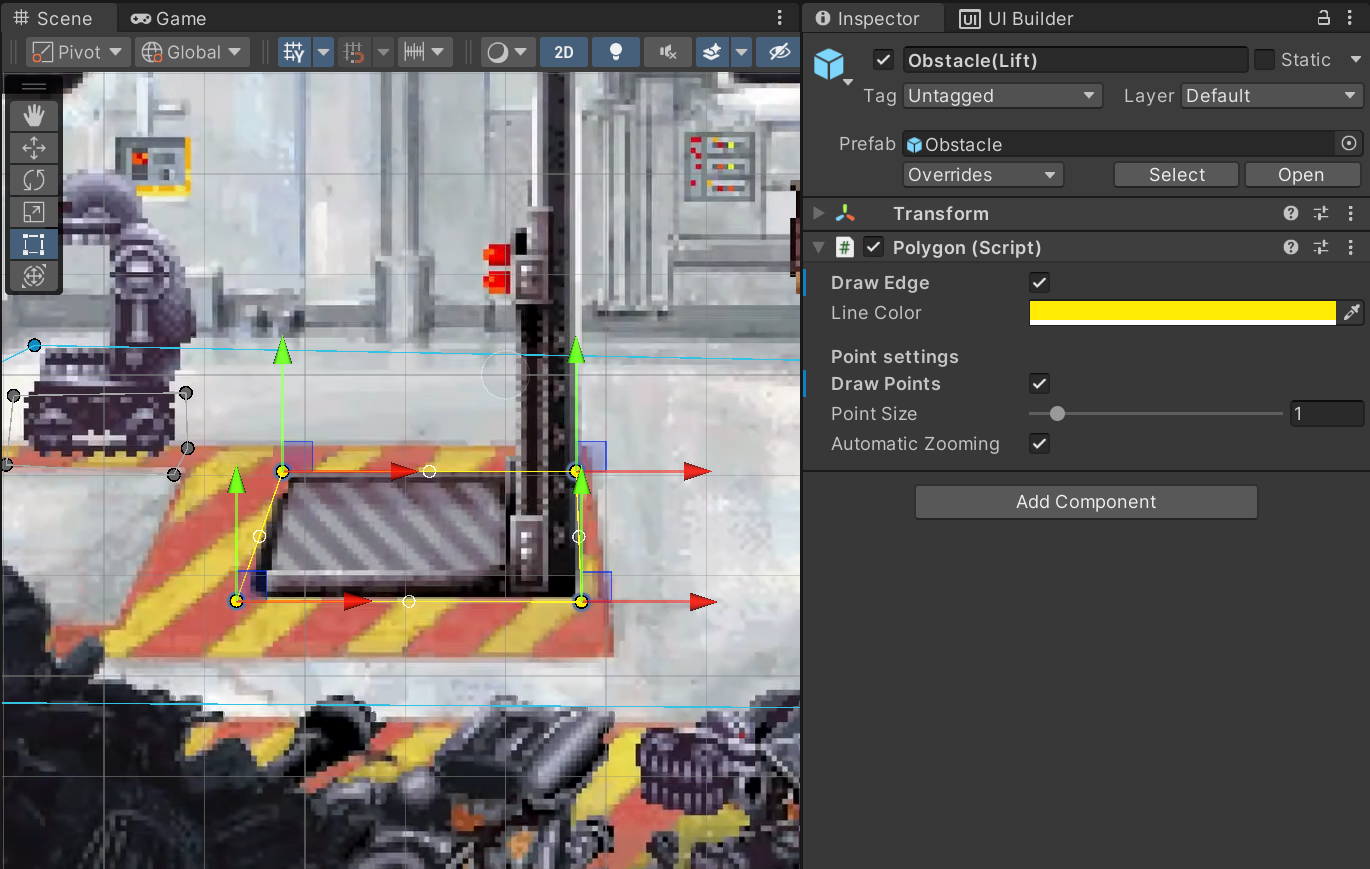
\includegraphics[width=1\linewidth]{img/User doc/polygon.png}
\caption{Polygon inspector.}
\label{fig:Manual-Polygon}
\end{figure}

\begin{figure}[H]
\centering
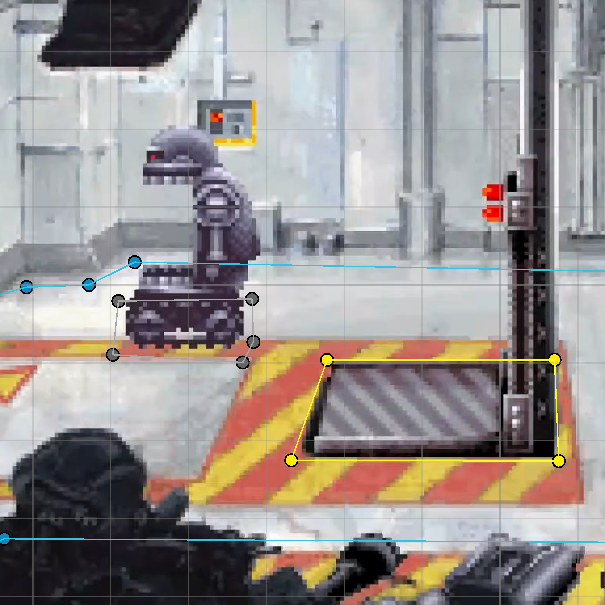
\includegraphics[width=.48\linewidth]{img/User doc/point_scaling.png}
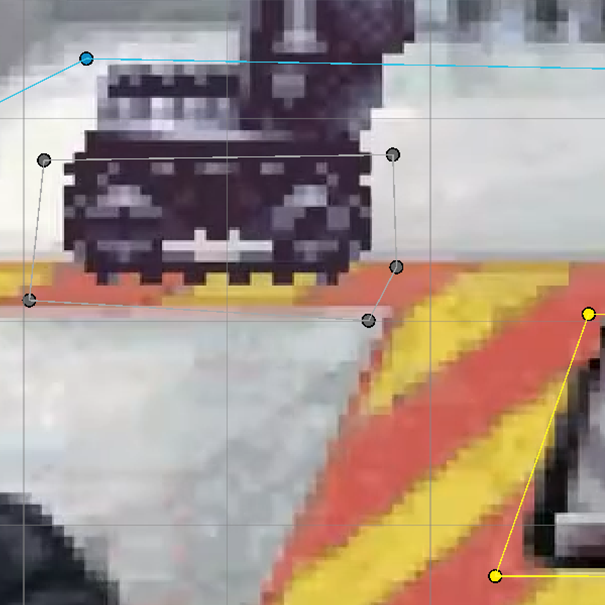
\includegraphics[width=.48\linewidth]{img/User doc/point_scaling2.png}
\caption{Point scaling based on zoom level.}
\label{fig:Manual-Zoom}
\end{figure}

\subsubsection{Character Movement \& Sprite Scaler}
The last two components of the walking system are \textbf{Character Movement} and \textbf{Sprite Scaler} scripts, whose application in the framework can be clearly seen in Figure \ref{fig:Manual-ChM&SS} for scene \textit{TSoMI}. 

The \textbf{Character Movement} script is attached to the player \verb|GameObject| or to any other character that requires movement in a walkable area. The script must be provided with a reference to the \textbf{Walkable Map}, and the desired movement speed can be configured. An optional end point may also be specified, primarily for debugging purposes. When defined, the graph in the \textbf{Walkable Map} component can visualize the path between the character's current position and the designated end point without entering play mode. This allows the user to interactively reposition the end point and verify that the polygonal navigation areas are configured correctly.

Finally, the \textbf{Sprite Scaler} component takes care of scaling the sprite of the object to which the component is attached. There are multiple options to choose from. The first option is \textit{None}, meaning no scaling is applied to the character. The other two options are \textit{X }and \textit{Y-based scaling}, where the scaling occurs based on the X or Y axis. The two borderline cases need to be selected, which define the scale the very top and bottom for Y axis or very left and right for X axis of the walkable area. The type of perspective can be also selected. If the \textit{Linear} option is enabled, the character scales linearly. The \textit{Hyperbolic} option provides more variety with the rate of scaling. The last scaling type is \textit{Custom}, which takes the scaling factor in each point in the component \textbf{Point} of the walkable polygon and interpolates between them based on the distance.
\begin{figure}[H]
\centering
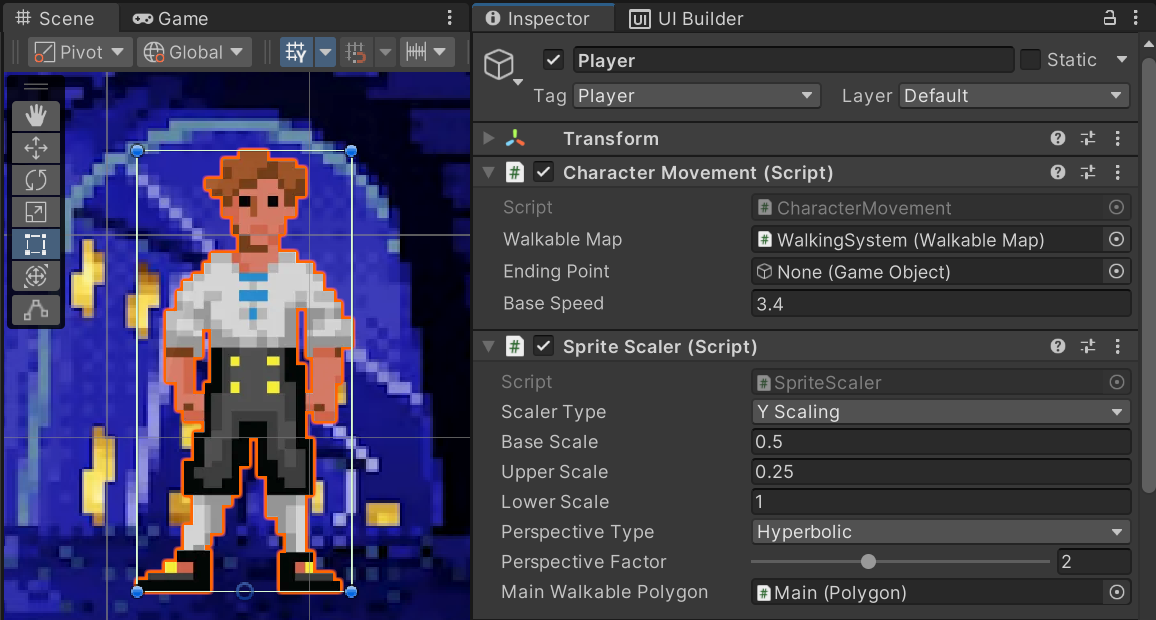
\includegraphics[width=0.8\linewidth]{img/User doc/character_movement.png}
\caption{Character Movement and Sprite Scaler inspector.}
\label{fig:Manual-ChM&SS}
\end{figure}

\subsection{Command System}
The Command system is complex and contains many components, so let us take a closer look at its individual parts.

\subsubsection{Command Manager}
The framework can instantiate a prefab in the hierarchy by navigating the menu options \verb|GameObject > Command System|. The prefab consists of a \verb|GameObject| with \textbf{Command Manager} script attached to it as a component (see an example of  the script from scene \textit{BaSS} in Figure \ref{fig:Manual-CM}). It takes the player \verb|GameObject| as a reference to apply action like walking to the appropriate location. The other two following properties \textit{Action Temp} and \textit{Action Sequence} are for debugging purposes as they display the currently hovered over object and the other game object that the player has interacted with.

\begin{figure}[H]
\centering
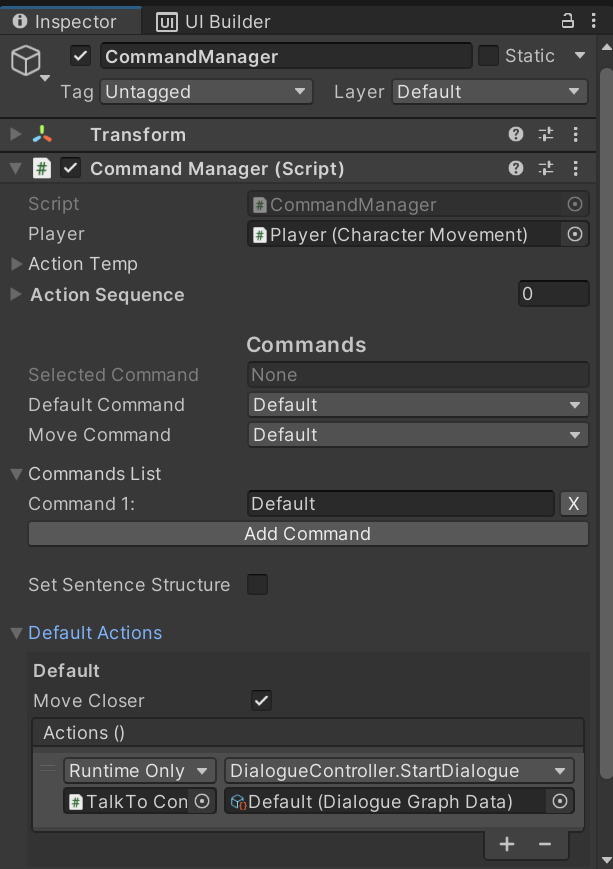
\includegraphics[width=.7\linewidth]{img/User doc/command_manager.png}
\caption{Command Manager inspector.}
\label{fig:Manual-CM}
\end{figure}

The next section, \textit{Commands}, is used to define the behavior associated with each command. All available commands are listed in the \textit{Commands List}. New entries can be added using the \textit{Add Command} button, while existing ones can be removed with the \textit{X} button next to each item. Editing commands in this list will automatically update all references across the framework’s inspectors without data loss. If there is a risk of losing data, the scripts provide separate buttons to synchronize the commands.

Above the list, there is a property displaying the currently selected command, primarily for debugging purposes. Additionally, the section includes options for setting the \textit{Default Command} and the \textit{Move Command}. The \textit{Default Command} determines which command will become active once the current action is completed. On the other hand, the \textit{Move Command} specifies the command responsible for detecting and responding to clicks related to character movement. The scene \textit{TSoMI} can serve as a useful reference for users, as it demonstrates a variety of commands and highlights the potential of this system.

Next is the \textit{Set Sentence Structure} option, which lets the developer define the structure that the command needs to follow when the command sentence is to be displayed. For example, Figure \ref{fig:Manual-CM3} shows a possible way to set this \textit{Sentence Structures}. \verb|Talk to| command is only followed by an object (e.g., Talk to customer), whereas \verb|Give| requires the "Object - Connector - Object" sequence (e.g., Give flower to customer).

\begin{figure}[H]
\centering
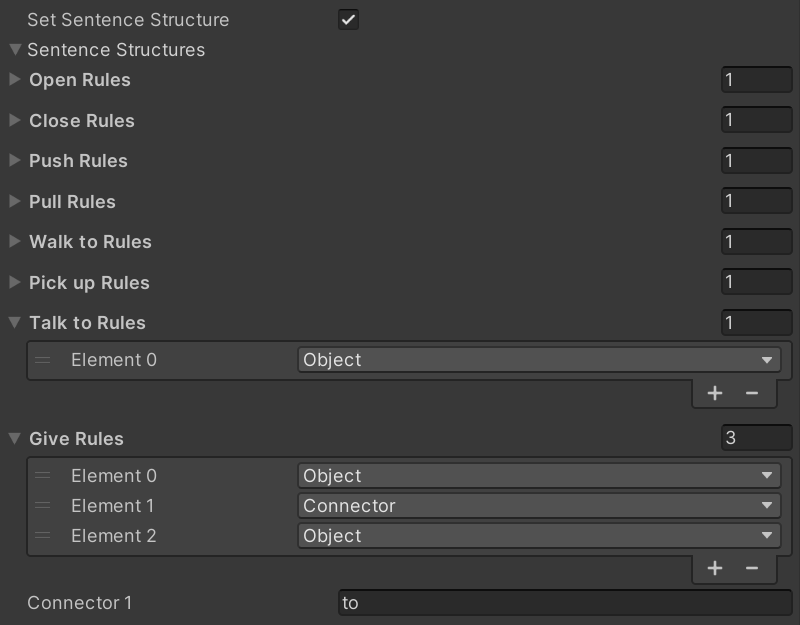
\includegraphics[width=.8\linewidth]{img/User doc/image_2025-07-04_203654317.png}
\caption{Command Manager inspector - Structure.}
\label{fig:Manual-CM3}
\end{figure}

Finally, the \textit{Default Actions} allow the developer to specify what should happen when all possible actions for a given object-command combination are invalid. This is useful for providing feedback to the player when their input is not correct and a different action is required. If the \textit{Move Closer} toggle is enabled, the character will walk up to the object before attempting to interact with it. The \textit{Actions} section below allows the developer to define additional behavior through Unity Events.

\subsubsection{World Object}
In order to create an interactable object in the scene, the user first needs to create a \verb|ScriptableObject| in the Assets folder by pressing right-click and selecting \verb|Create > Item > World Item|. Here, the user can define the name as well as the description of the item. This asset helps to reference the item throughout the whole project, even in other scenes. Features such as the sprite or what the item does when interacted with needs to be set in the \verb|GameObject| with the component \textbf{World Object} attached to with a possible implementation in Figure \ref{fig:Manual-WO} from the \textit{BaSS} scene. 

\begin{figure}[H]
\centering
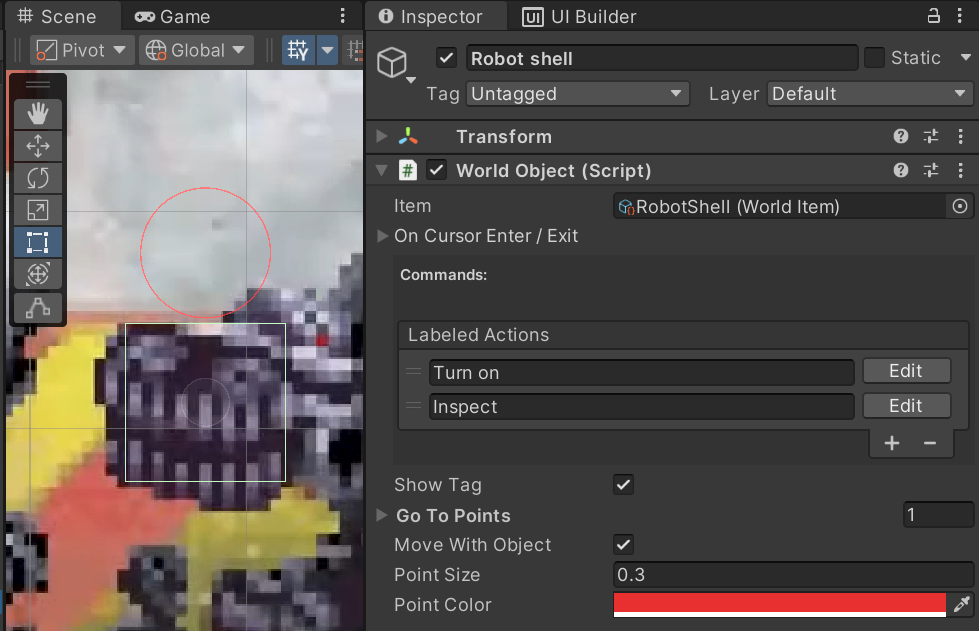
\includegraphics[width=.8\linewidth]{img/User doc/world_object.png}
\caption{World Object inspector.}
\label{fig:Manual-WO}
\end{figure}

The script takes a \textbf{World Item} asset as a reference in order to assign the item with the actions defined. Except for an option to show a tag with a name of the object, the script also offers a way to define the position of the player when interaction is initiated. The can define multiple of these so-called \textit{Go To Points} using 2D vector coordinates and during runtime the closest of them is chosen. If none are defined and the character is ordered to move to that position, it selects the position of the object itself. If the object changes position (it is a moving character, for example), the user can define if the position of these points is relative to the object or not. There are also visual settings like selecting a color and the size of the circle defining the point.

The desired behavior can be created in the reorderable \textit{Labeled Actions} list. If the player interacts with the given object, the command system goes one by one in the list and if all required conditions are met, the given action is executed. When creating a new action using the \textit{+} button, the user can set a label to that action. This label is purely visual and serves to make the editing of actions readable. When the \textit{Edit} button is pressed, a window pops up, which serves to create the logic of an action. The window first starts with \textit{Previous Interactables}. If enabled, the action is required to contain the same actions as the player had previously interacted with, which can be seen in \textit{Action Sequence} in \textbf{Command Manager}. The next step in verification are \textit{Conditions}, which is a list of \verb|ScriptableObject| \textbf{Variables}, which can be created in the Assets folder through the \verb|Create > Variable > ...| option. This lets the user define either an integer, a float, a string or a boolean variable. In the action window, the conditions need to be given the expected value. If the \textit{Conditions} or the \textit{Previous Interactables} do not match, the action is considered invalid and the next action in the list is checked. In case everything matches, the \verb|UnityEvents| from the very bottom of the window are called based on the type of the click.

\begin{figure}[H]
\centering
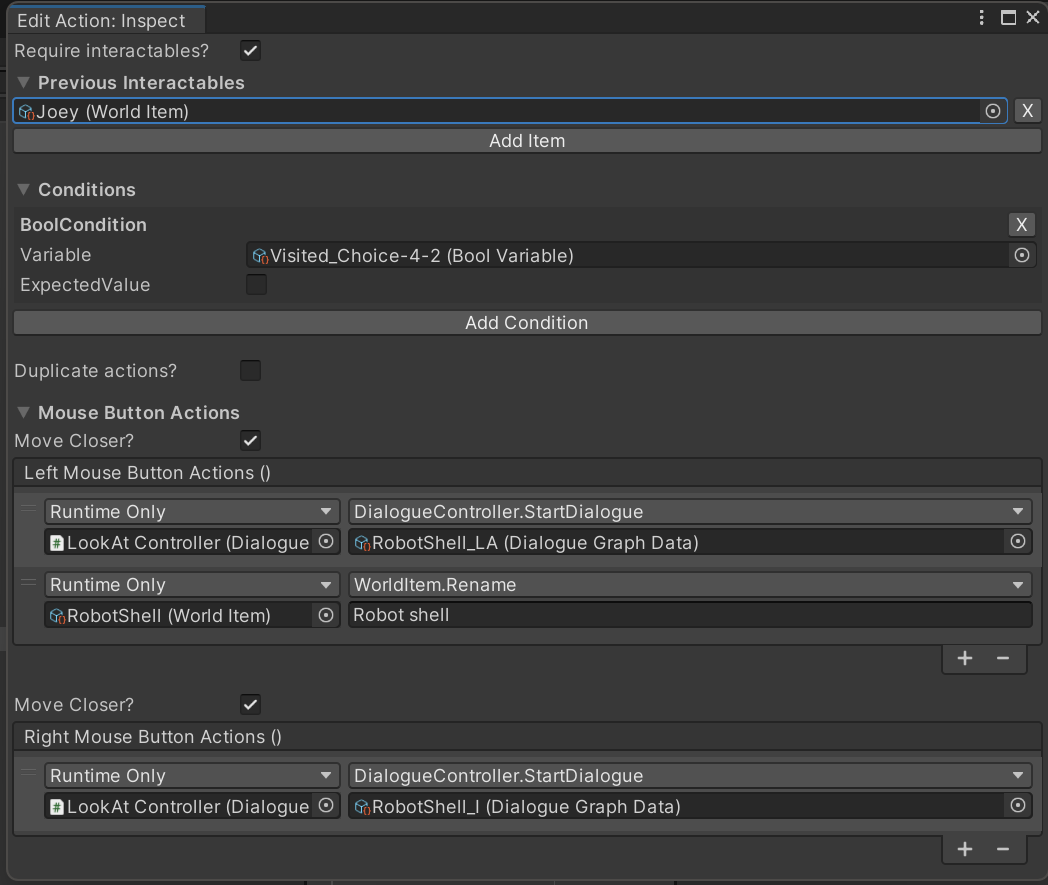
\includegraphics[width=.8\linewidth]{img/User doc/action_window.png}
\caption{Action window.}
\label{fig:BaSS-manual}
\end{figure}

\subsubsection{Inventory Object}
\textbf{Inventory Objects} are interactables inside the player's inventory. Unlike \textbf{World Objects}, they cannot be assigned actions that easily, since sometimes the player needs to use an item in another scene and doing so would require the developer to create a new instance of the same item in every scene. We want to make working with our framework easy and intuitive. So we decided to create a \textbf{Slot Manager} in every scene, which would manage the actions of inventory slots in the current scene (see Figure \ref{fig:Manual-SM}). Defining actions is the same as for \textbf{World Objects}, but first the developer needs to create a new slot using the \textit{Add Slot} button. Then, they need to assign the actions to an item using \verb|ScriptableObject| Inventory Item, which can be created by right-clicking in the Assets folder and selecting \verb|Create > Item > Inventory Item|. Similar to \textbf{World Item}, the developer can set the name as well as the description of the item. In addition, there is an option to add a sprite. This feature is used when the inventory is icon-based, more on that in Section \ref{UD-IS}.


\begin{figure}[H]
\centering
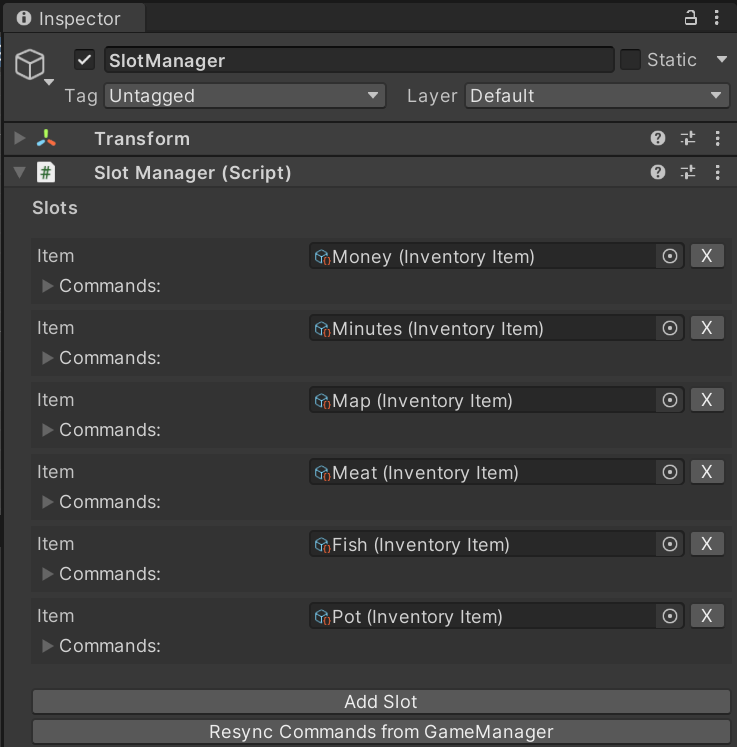
\includegraphics[width=.7\linewidth]{img/image_2025-07-05_133040354.png}
\caption{Slot Manager with six slots for Inventory Items.}
\label{fig:Manual-SM}
\end{figure}

To ensure that an inventory slot appears correctly in the inventory and has expected behaviors, such as being draggable by the mouse cursor or displaying a tag when hovered over, a prefab must be created. This prefab acts as a reusable template, allowing the system to instantiate inventory slot elements automatically, each with the required components and behaviors already configured. Once the prefab is properly set up, the developer does not need to manually configure each inventory slot instance.

The TaleCraft framework provides a ready-made implementation of such an inventory slot prefab, as demonstrated in the \textit{TSoMI} and \textit{BaSS} example scenes. In order for the framework to access and instantiate this prefab, it must be registered in the \textbf{Prefab Library} under the label \textit{InventorySlot}.

Since inventory slots are part of the user interface (UI), the system for handling input, such as clicking or dragging, differs from that used for \textbf{World Objects}. Moreover, \textbf{World Objects} typically only respond to left or right mouse clicks, whereas inventory interactions may include additional behaviors such as dragging. These behaviors must be defined by the developer, but the TaleCraft framework simplifies the process.

Unity provides the \textbf{Event Trigger} component, which can be attached to a \verb|GameObject| to define responses to various input events, such as cursor entry or exit, clicks, drags, and more. In the TaleCraft framework, inventory slots make use of this system in the provided demonstration scenes. To help manage input more precisely, the framework includes the \textbf{Custom Pointer Handler} component, which distinguishes between left and right mouse button inputs.

Additionally, the framework offers a \textbf{Trigger Setter} component, which defines a set of commonly used methods for inventory interactions. These include features such as dragging items or displaying tags when the mouse hovers over a slot, which streamlines the implementation of standard inventory behaviors. All of this can be examined further in scenes \textit{BaSS} and \textit{TSoMI}.

\subsection{Inventory System}
\label{UD-IS}
The inventory system provides the necessary functionalities to manage and display the inventory. Figure \ref{fig:Manual-Inventory} presents a possible use of the \textbf{Inventory Manager} script, which takes care of basic functionalities like taking and removing objects from the inventory. The component can be attached to the player and has the option to define the limit of items that can be picked up. Finally, the user can define the contents of the inventory in the list called \textit{Inventory}. It contains entries of type Inventory Item, which can be defined in the Assets folder by pressing right click and selecting \verb|Create > Item > Inventory Item|. The newly created \verb|ScriptableObject| can be given a name, description, as well as rendering data such as a sprite if the icon of the inventory item is meant to be displayed. The item can be dragged as a new entry into the inventory.
\begin{figure}[H]
\centering
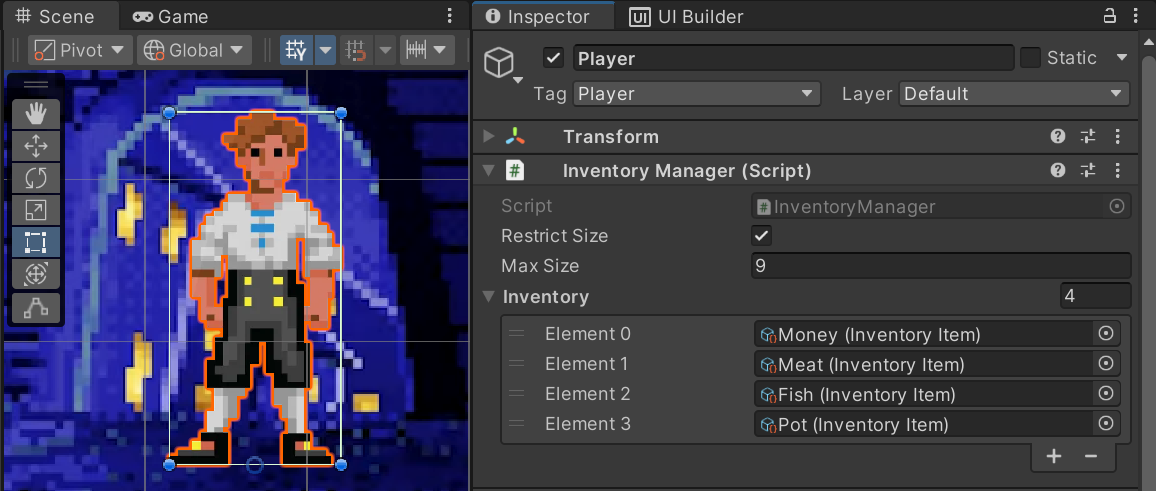
\includegraphics[width=.8\linewidth]{img/User doc/inventory.png}
\caption{Inventory Manager inspector.}
\label{fig:Manual-Inventory}
\end{figure}

Another component that takes care of visualizing the inventory is \textbf{Display Inventory}. There is an option to set between two types of inventory: \textit{Name} or \textit{Icon}. The former displays the inventory items as a label with the word (or their combination), whereas the latter creates an icon depicting the item. Both of these approaches are used in the \textit{BaSS} and \textit{TSoMI} scenes.

Afterwards, the layout settings can be seen. These can adjust the configuration of the inventory slots: the starting location, width, height and more. 

Finally, the \textit{Max Item Count} option sets how many items can be visible at most. It ties directly to the last script in the inventory system called \textbf{Inventory Scroll Button}, which when attached to a \verb|GameObject| lets the user define the behavior of scrolling through the inventory by pressing an arrow. This exact scenario is used in \textit{TSoMI} scene.

\subsection{Dialogue System}
The dialogue system provides the necessary tools for creating and managing conversations between characters. Dialogues are represented as dialogue graphs, which can be created in the Assets folder by right-clicking and selecting \verb|Create > Dialogue > Dialogue Graph|. Once opened, the asset displays a dedicated editor window, as shown in Figure \ref{fig:Manual-DW}.

\begin{figure}[H]
\centering
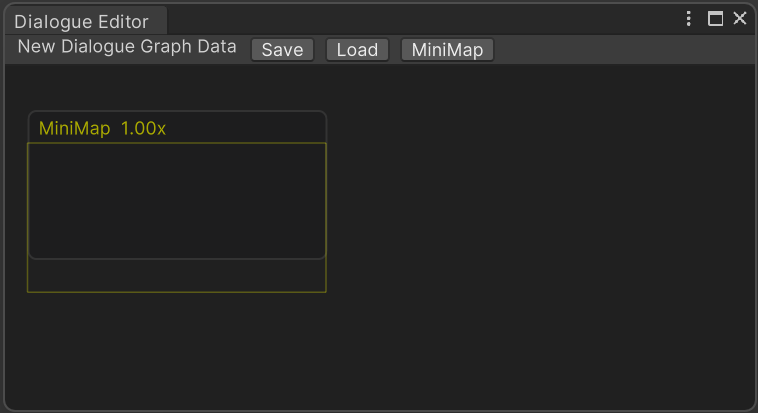
\includegraphics[width=0.8\linewidth]{img/User doc/image_2025-07-04_123651622.png}
\caption{Dialogue graph window.}
\label{fig:Manual-DW}
\end{figure}

At the top of the window is a panel that displays the file name along with three buttons. The first, \textit{Save}, stores the current state of the graph. If the window is closed without pressing this button, any unsaved changes will be lost. The second button, \textit{Load}, reloads the last saved version of the graph. This means any edits made since the last save will be discarded. The third button, \textit{MiniMap}, toggles the visibility of a small map in the top-left corner of the editor window, which provides an overview of the graph layout.

\subsubsection{Nodes}
To add elements to the dialogue graph, the user must press the Space key, which opens a search window. This interface allows the creation of either a \textit{Node} or a \textit{Group}. Selecting the \textit{Node} option presents six different node types to choose from. All node types support naming and include the option to generate a corresponding boolean variable called \textit{Visited}. This variable tracks whether the node has been accessed during a conversation, enabling conditional behaviour based on the history of dialogues.

A new Visited variable can be created by clicking the "\textit{+}" button next to its field in the node's configuration. The asset is automatically stored at the following path: \verb|Assets/Variables/Visited/[GraphName]|, where \verb|[GraphName]| corresponds to the name of the dialogue graph. The filename of the Visited variable is either the node’s custom ID (if specified) or its unique GUID. For this reason, it is recommended to assign an ID to the node before creating the Visited variable. Otherwise the nodes have a very different structure from one another. In the rest of this Section, each type of node will be closely examined with Figures \ref{fig:Manual-Nodes1} and \ref{fig:Manual-Nodes2} providing visual guidance.

\begin{itemize}
    \item The \textbf{Start node }is a straightforward element in the dialogue graph. Aside from allowing the assignment of an ID and a corresponding \textit{Visited} variable, it features a single output port. Only one Start node is required per graph, any additional Start nodes present will be ignored. This node functions only as an entry point, indicating where the dialogue begins within the graph.
    \item In addition to the basic functionality common to all nodes, the \textbf{Event node} includes an \textit{Add Event} button. As the name implies, clicking this button adds a new slot for an associated \textbf{EventScriptableObject}, which references a \verb|ScriptableObject| used to trigger events. Since dialogue graphs are assets and cannot directly reference scene objects, this mechanism establishes the necessary link between the dialogue system and the game scene. A dialogue event \verb|ScriptableObject| can be created via the menu path: \verb|Create > Dialogue > Dialogue Event|. To bind this \verb|ScriptableObject| to the scene, a \verb|GameObject| in the scene must include the \textbf{Event Listener} component. This component maintains a list of pairs, where each pair consists of an event \verb|ScriptableObject| and a corresponding Unity Event that is invoked when the event is triggered. 
    \item The \textbf{Branch node} enables conditional branching, which allows the conversation flow to change based on the defined criteria. A new condition can be added by clicking the \textit{Add Condition} button and selecting one of four available types: boolean, integer, float, or string. Afterwards, a new field appears at the bottom of the node, which allows the user to specify the expected value for that condition. The node includes two output ports labeled \textit{True} and \textit{False}. If all defined conditions are satisfied, the graph continues along the \textit{True} output. If any condition fails, the flow proceeds through the \textit{False} output instead. 
    \item The \textbf{Dialogue node} provides the actual lines of dialogue spoken by characters. Initially, the node contains a single input and output port, as well as a setting labeled \textit{Continue Style}. The user can choose between two options: \textit{Wait} or \textit{Button}. The \textit{Wait} option allows the user to specify a duration (in seconds) for which the dialogue remains on screen before automatically continuing. The \textit{Button} option, on the other hand, enables the user to define a button that, when clicked, progresses the dialogue.

Additional dialogue entries can be added using the \textit{Add Text} button. Each entry consists of a pair: a \textit{Character ID} and a \textit{Dialogue Text} field. The \textit{Character ID} takes a reference to a \verb|ScriptableObject| of type \textbf{CharacterID}, which can be created by right-clicking in the Assets folder and selecting \verb|Create > Dialogue > Character ID|. This object allows configuration of the character's name, text offset (in \verb|Vector2|), and text color—settings that control how the text is displayed on screen. The actual binding of the ID to a specific \verb|GameObject| in the scene is explained later in this section. The \textit{Dialogue Text} field contains the line spoken by the character associated with the selected ID.

The Dialogue node also supports branching through dialogue choices. By clicking the \textit{Add Choice} button, additional output ports are generated. These are used exclusively to connect to \textit{Choice} nodes, which enable the player to select from multiple dialogue options during gameplay.

    \item The \textbf{Choice node} connects exclusively to additional output ports of a Dialogue node and is used to present clickable options to the player during dialogue sequences. It contains a text field where the developer specifies the content of the choice that will be shown on screen. Similar to the Branch node, the Choice node allows the addition of conditions that determine whether the choice is visible or interactable during gameplay. 
    \item  The final node type is the \textbf{End node}, which is responsible for terminating the dialogue flow. It offers three options: ending the conversation entirely, repeating the last Dialogue node, or returning to the Start node. Regardless of the selected behavior, the End node does not contain any output ports, since it marks the end of a given dialogue path. 
\end{itemize}
\begin{figure}[H]
\centering
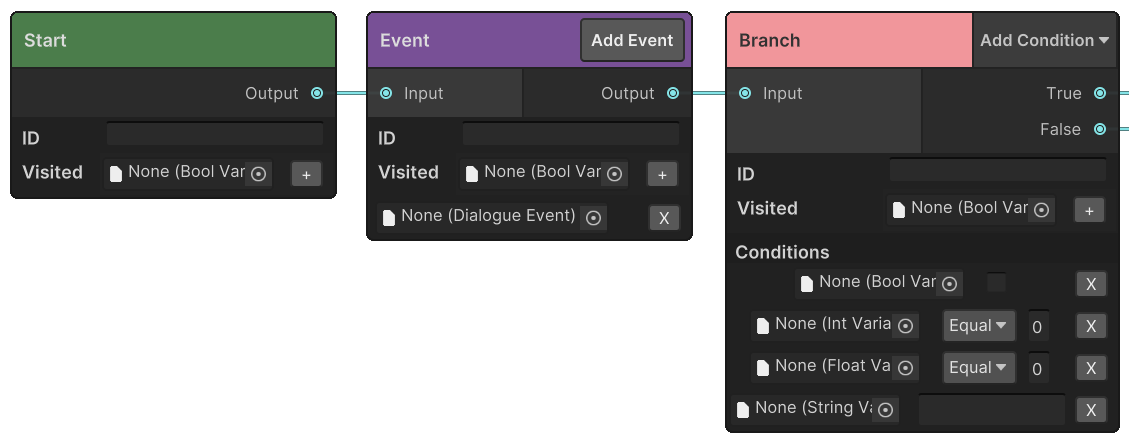
\includegraphics[width=1\linewidth]{img/User doc/nodes1.png}
\caption{Start, Event and Branch nodes.}
\label{fig:Manual-Nodes1}
\end{figure}
\begin{figure}[H]
\centering
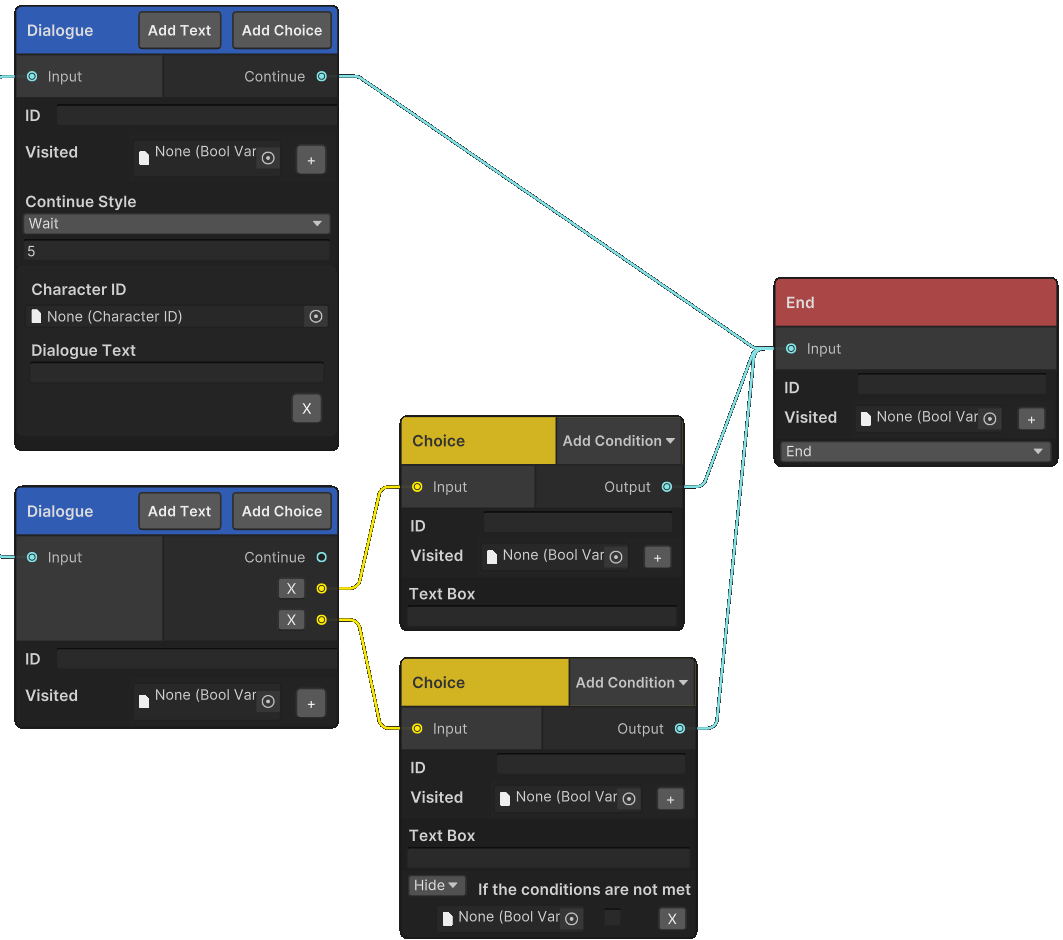
\includegraphics[width=1\linewidth]{img/User doc/nodes2.png}
\caption{Dialogue, Choice and End nodes.}
\label{fig:Manual-Nodes2}
\end{figure}

Both the \textit{TSoMI} and \textit{BaSS} scenes use the dialogue system, and it is recommended to examine the dialogue graphs created for these showcase scenes, as they provide practical examples of how the system can be used. 

\subsubsection{Groups}
If the user chooses to create a new group from the search window via the path \verb|Groups > Base group|, a new box titled \textit{Dialogue Group} will appear in the editor. Nodes can be added to the group by clicking and holding the left mouse button on a node, dragging it into the group area, and then releasing the button. Multiple nodes can be added to a single group, and it is possible to create connections between any nodes, even those outside the group. When a node is part of a group, moving the group box will also move the contained nodes accordingly. To remove a node from the group, the node needs to be dragged outside of the group while holding Shift key. A group can be renamed by double-clicking on its title. 

\subsubsection{Dialogue Control}
In order to run a conversation, the scene must contain a \verb|GameObject| with the \textbf{Dialogue Controller} component attached. This component is responsible for initiating the dialogue and also triggers Unity Events defined in its Inspector both at the beginning and at the end of the conversation. 

Using a Dialogue node, the user can associate a line of text with a specific character through a \textbf{CharacterID} asset. To establish the link between a \verb|GameObject| in the scene and ensure that the dialogue text is displayed near the correct character, the \textbf{Dialogue Controller} component provides a list called \textit{Character ID Data}. Each entry in this list maps a \verb|GameObject| (referred to as the \textit{Character}) to a corresponding \textbf{CharacterID} asset (referred to as the \textit{ID}).

The \textbf{Dialogue UI Controller} component allows the developer to assign a specific prefab to be instantiated as the dialogue text box during runtime. Additionally, it provides options in the Inspector for customizing UI elements, such as button colors and other minor interface settings.

\section{Showcase}
To demonstrate the capabilities of our framework, we chose to recreate scenes from two classic point-and-click adventure games: \textit{The Secret of Monkey Island} and \textit{Beneath a Steel Sky}. Both titles are iconic representatives of the genre, released during its golden era, and introduced several innovative features that later became genre standards. While \textit{The Secret of Monkey Island} uses a command-based interaction system, \textit{Beneath a Steel Sky} takes a more context-sensitive approach. The two games also differ in their inventory design and other small UI elements, such as interaction tags and descriptive sentences, making them ideal candidates to test and showcase the flexibility of our framework.

Another reason we selected these specific titles is their age and current distribution status: they are no longer sold as new releases. Works in the public domain can be used freely without restrictions, but since video games are still a relatively young medium, only a few very old titles or special cases have entered the public domain.
Our framework is non-commercial and our use of these games falls under fair use for educational purposes, but the boundaries of fair use are not always clearly defined. 
Newer game developers might object to similar use of their intellectual property. We therefore encourage all readers to support the original games where possible. The sequel to \textit{Beneath a Steel Sky} is available on Steam, and \textit{The Secret of Monkey Island} can be purchased as a modern remake.

\subsection{Instructions}
The \verb|Build| folder inside \verb|Attachments.zip| includes the \verb|TSoMI-Build| and \verb|BaSS-Build| directories, which in addition to a few application binaries, a dynamically linked library and directories with the game assets contain an executable file. To run the game, simply run the \verb|TaleCraft.exe| binary. Both games will show a \textit{Made with Unity }splash screen followed by the scene itself. To quit the game, one needs to simply press Esc on the keyboard.

\subsection{Beneath a Steel Sky}
\textbf{Beneath a Steel Sky} showcase takes place in a starting location of the original game. The style of the following instructions are taken from the original manual for the game \cite{BaSS-Manual}.

\textbf{Clicking} on objects or characters causes the main character, Foster, to interact with them. To \textbf{move} Foster, the player can point the cursor at navigable areas of the screen and click either mouse button. Foster will not walk into walls or inaccessible areas. Certain objects in the game world can be \textbf{examined} or \textbf{interacted} with. These are identified by on-screen tags that appear when the cursor hovers over them. Pressing the \textbf{left mouse button} causes Foster to examine the object, while the \textbf{right mouse button} attempts to pick up or use it. The game selects the most logical action based on context, for example, clicking on a character will typically initiate a conversation. 

When the pointer is moved to the top edge of the screen, a horizontal bar appears, which represents an \textbf{inventory} (see Figure \ref{fig:BaSS-manual}). It contains items currently carried by Foster and interaction with them follows the same logic as with objects in the game world: \textbf{hovering} the cursor over an item reveals its name, pressing the \textbf{left mouse button} displays a short description of the item, while pressing the \textbf{right mouse} button selects it for further interaction. 

When the cursor hovers over another character, clicking either mouse button initiates a conversation. Dialogue options are presented at the top of the screen and the player can choose a line by clicking on it. 

\begin{figure}[H]
\centering
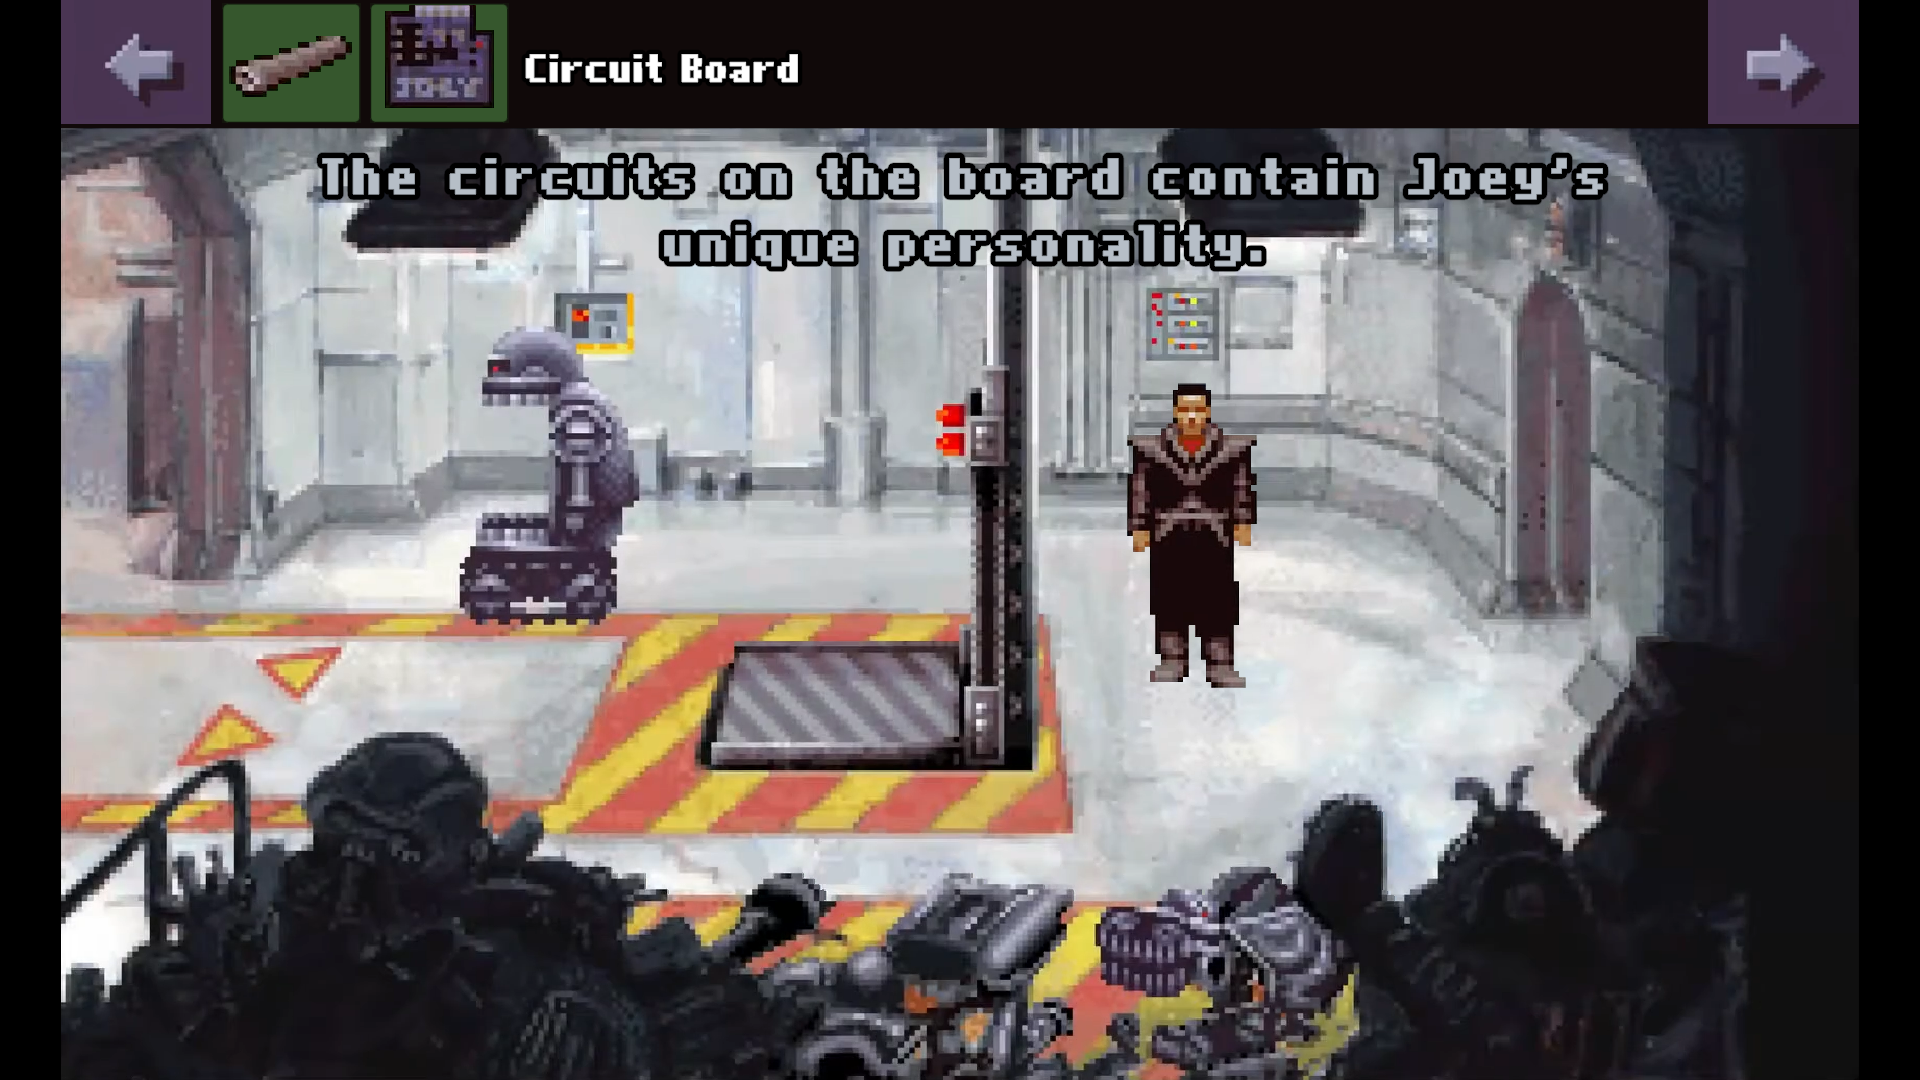
\includegraphics[width=.8\linewidth]{img/manual.png}
\caption{Beneath a Steel Sky (showcase): Screen.}
\label{fig:BaSS-manual}
\end{figure}

\subsection{The Secret of Monkey Island}
The showcase game of The Secret of Monkey Island takes place on a street in the Town of Maleé. The style of the following instructions are taken from the original manual for the game \cite{TSoMI-Manual}.

\subsubsection{Screen}
The game screen is divided into multiple visually distinct parts (see Figure \ref{fig:TSoM-manual}):
\begin{enumerate}
    \item \textbf{Animation window} is the largest area of the screen and serves as the main stage where the action occurs. It displays the current location the protagonist, Guybrush, is currently in. All character dialogue and game-related messages are also displayed in this window. 
    \item Located directly below the Animation window, the \textbf{Sentence} is where players construct simple commands that guide Guybrush's actions. A typical sentence includes a verb and one or two objects. For example, a valid command might be: “\verb|Look at poster.|”
    \item \textbf{Command verbs} are listed in columns underneath the Sentence. Players select verbs by hovering the cursor over them and clicking the left mouse button.
    \item The \textbf{Inventory} is located to the right of the Command verbs section. There is no limit to how many items can carried. When more than six items are in the inventory, arrow buttons appear to allow scrolling through the full list. 
\end{enumerate}

\begin{figure}[H]
\centering
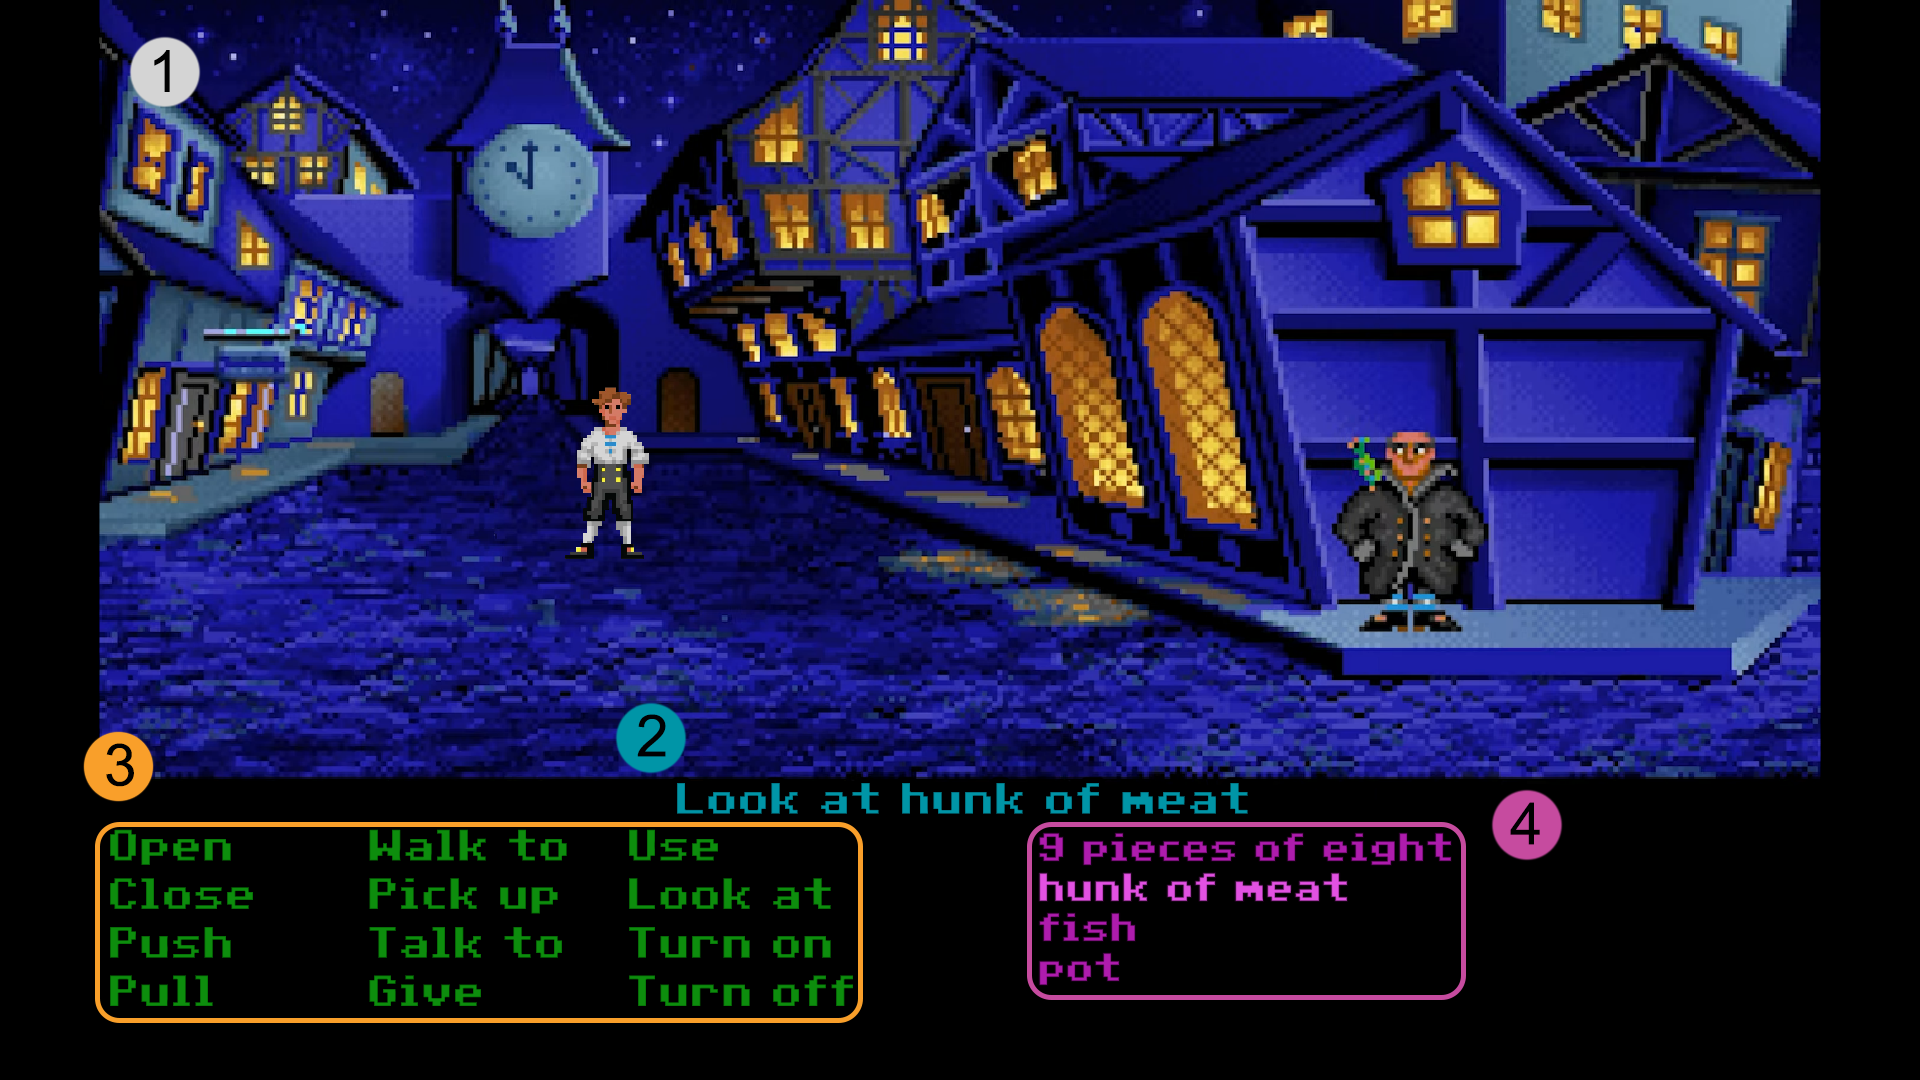
\includegraphics[width=.8\linewidth]{img/tutorial-tsomi.png}
\caption{The Secret of Monkey Island (showcase): Screen.}
\label{fig:TSoM-manual}
\end{figure}

\textbf{Noun Selection and Character Interaction}
Objects, also referred to as nouns, can be selected in two ways. The most common method is by moving the cursor over an object in the Animation window. Most interactive objects in the environment have names, and if an object is usable, its name will appear in the Sentence when the player hovers over it. If no name appears, the object is likely part of the background and serves no gameplay purpose. The objects from the Inventory can be selected directly by clicking on them.

\subsubsection{Movement}
To move Guybrush around the world, the cursor needs to be pointed to the desired location followed by a click. \textit{Walk to} is the default verb in the Command sentence, as moving is the most frequent action players will perform.

\subsubsection{Talking to Characters}
To talk to another character, the player can move the pointer over them and press the right mouse button. During a conversation, dialogue options will appear at the bottom of the screen as seen in Figure \ref{fig:TSoM-manual2}.  The phrase that we want Guybrush to say can be selected by simply clicking on it. What Guybrush says can influence how other characters respond, and new dialogue options may appear as conversations develop.

\begin{figure}[H]
\centering
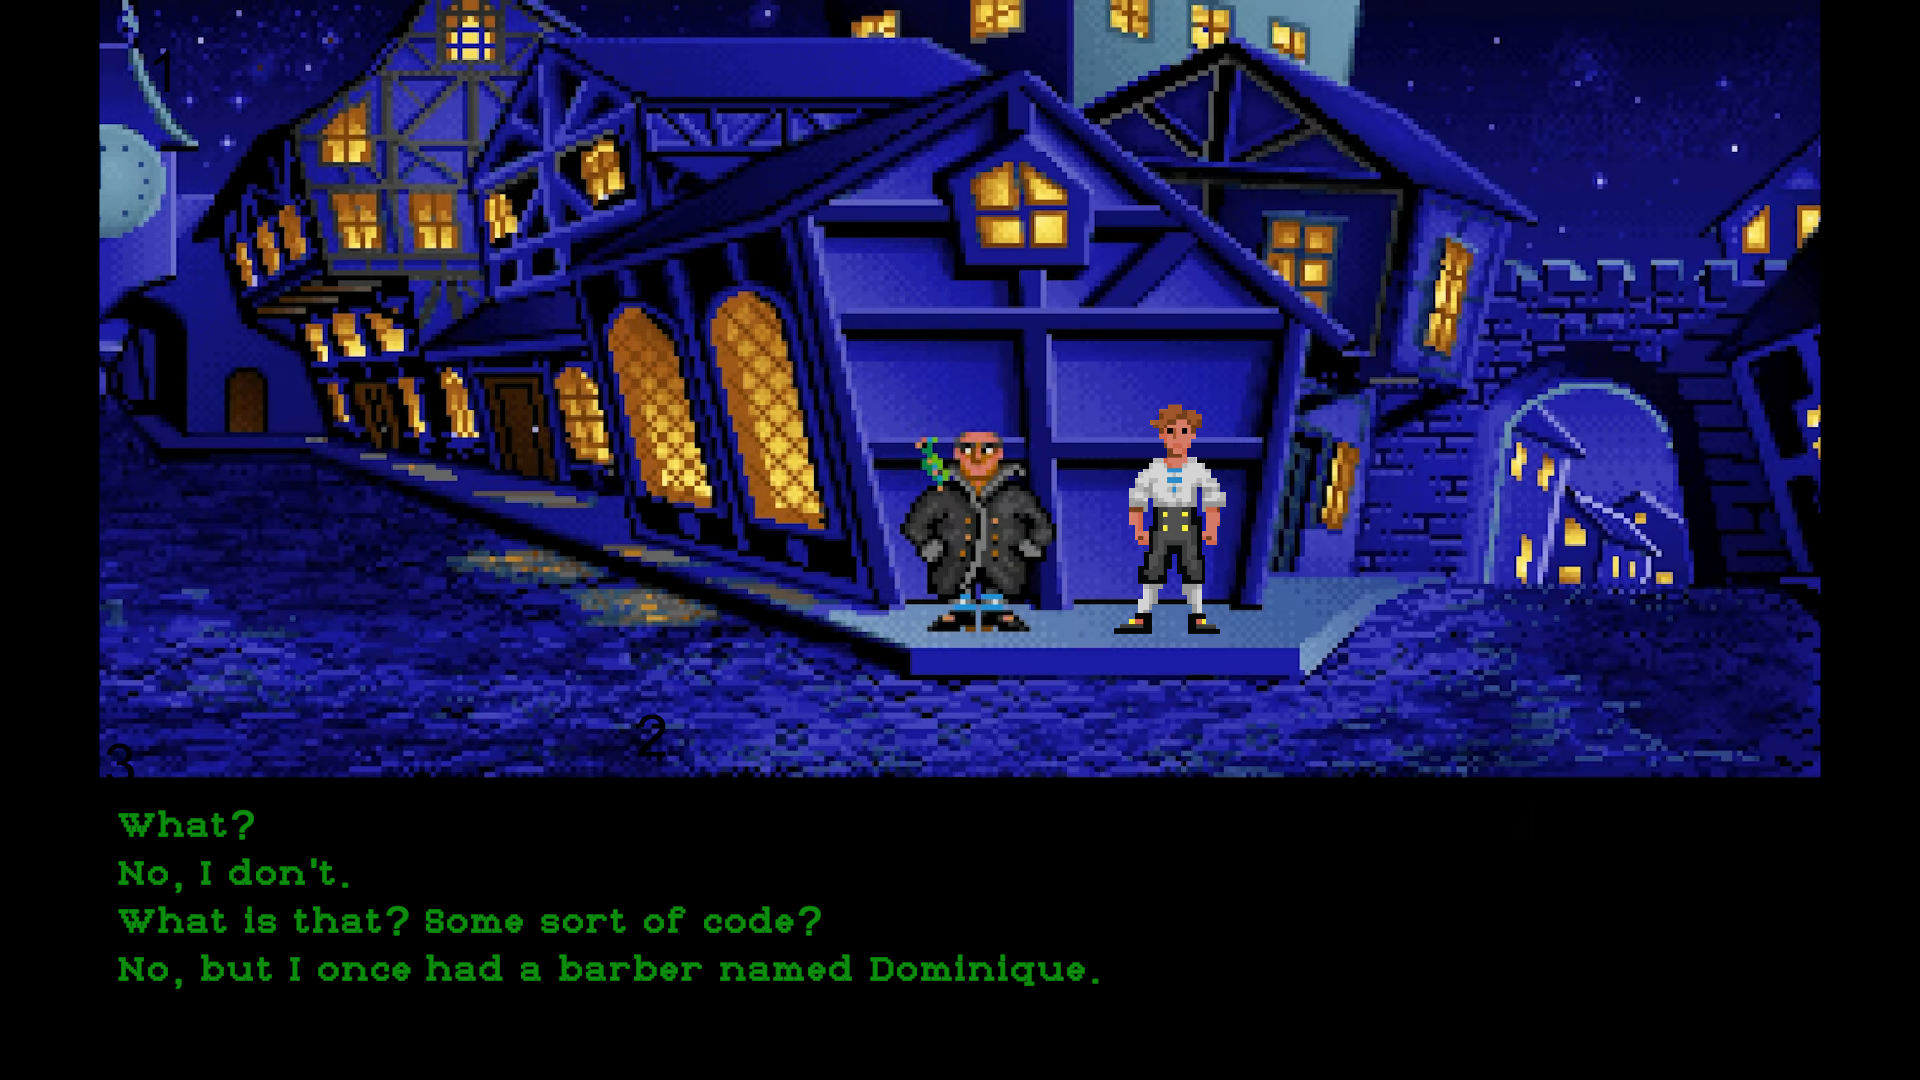
\includegraphics[width=.8\linewidth]{img/manual-tsomi.png}
\caption{The Secret of Monkey Island (showcase): Dialogue.}
\label{fig:TSoM-manual2}
\end{figure}